\section{Part 2: Cross-Validation}
	\begin{table}[ht]
		\centering
		\begin{tabular}{@{}ll@{}}
			\toprule
			\textbf{Variable}       & \textbf{Description}                        \\
			\midrule
			HR features             & Mean, median, std, min, max, AUC of the HR signal  \\
			Round                   & Puzzle round (1–4)                          \\
			Phase                   & Phase within each round (1–3)               \\
			Individual               & Participant ID                              \\
			Role                    & Puzzler or instructor                       \\
			Frustration             & Self‐rated frustration (0–10)               \\
			Cohort                  & Cohort ID (D11, D12, D13)                   \\
			\bottomrule
		\end{tabular}
		\caption{Key variables in the HR\_data.csv subset.}
		\label{tab:dataset_variables}
	\end{table}

	\subsection{Feature Selection and Preprocessing}
	As specified in the task description, only the hart rate data will be used for the classification task.
	This the following attributes will be used: HR Mean, HR Median, HR std, HR Min, HR Max, HR AUC\@.
	The data will be standardized and normalized to ensure that all features contribute equally to the model training.

	The Frustration variable will be used as the target variable having values from zero to eight, however, the values
		6 and above will be grouped into one class (high frustration) due to the small number of samples in these
		classes.

	\subsection{Machine Learning Models}
	Two machine learning models will be used for the classification task:
		Logistic Regression, XGBoost and a baseline classifier that predicts the most common label.
	Logistic Regression is chosen for its simplicity and interpretability, while XGBoost is selected for its
		ability to handle non-linear relationships and its strong performance in classification tasks.
	These models will output class probabilities for each frustration level, allowing for a multi-class classification
		task.

	\subsection{Cross‐Validation Scheme}
	To ensure that the models generalize well to unseen data, a two-level cross-validation scheme will be employed.
	The inner fold will use stratified group 3-fold cross-validation, ensuring that each fold contains a representative
		sample of each frustration level.
	The outer fold will use Leave-One-Group-Out Cross-Validation, where each group is defined by the Individual ID\@.
	This approach ensures that no individual is present in both the training and test sets, preventing data leakage and
		ensuring that the model can generalize to new individuals.
		
	In the inner fold the models will be tested on different hyperparameters to find the best performing model.
		The hyperparameters for the Logistic Regression model will be the regularization strength.
		For the XGBoost model, the hyperparameters will include the learning rate, maximum depth of trees, and n\_
		estimators (number of trees) and reg\_lambda (L2 regularization term).


	\subsection{Statistical Comparison of Models}
	To compare the performance of the models across the folds, a repeated-measures ANOVA will be conducted.
		Repeated-measures ANOVA is appropriate here because it accounts for the non‐independence of observations
	within each fold.
	The ANOVA can be seen in \autoref{tab:anova_results}.
	Even though the p-value is not significant, it is close to the threshold of 0.05, indicating that there may be a
		chance of a difference in performance between the models.

		\begin{table}[ht]
			\centering
			\begin{tabular}{@{}lrrrr@{}}
				\toprule
				\textbf{Source} & \textbf{F} & \textbf{Num DF} & \textbf{Den DF} & \textbf{Pr $>$ F} \\
				\midrule
				Model           & 3.3137       & 2               & 26               & 0.0522            \\
				\bottomrule
			\end{tabular}
			\caption{Results of the repeated-measures ANOVA comparing model performance across folds.}
			\label{tab:anova_results}
		\end{table}


	To check the normality of the residuals, QQ plots will be used. In \autoref{fig:qqplot} the QQ plot shows that
		the residuals are somewhat normally distributed, which is a key assumption for the ANOVA test.
		However, there are some deviations from normality, particularly in the tails of the distribution.

	\begin{figure}
		\centering
		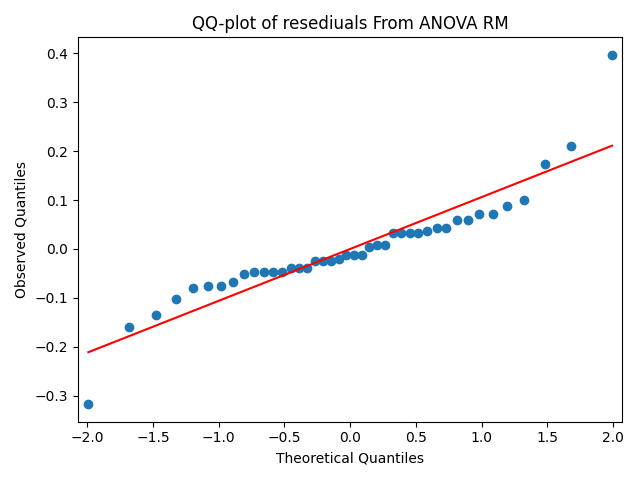
\includegraphics[width=0.7\textwidth]{Part2/qqplot}
		\caption{}
	    \label{fig:qqplot}
	\end{figure}

	To control the family-wise error rate when performing multiple comparisons, Holm's stepdown correction will be
		applied.
		This method is a stepwise procedure that adjusts the p-values of multiple tests to reduce the likelihood of
	false positives.

		\begin{table}[ht]
 \centering
 \sisetup{
  table-format = -1.3,     % for T values (can be negative)
  round-mode    = places,
  round-precision = 3,
 }
 \begin{tabular}{
  l                             % Comparison
  S[table-format=2.3]           % T statistic
  S[round-precision=0]          % df
  S[table-format=1.3]           % p (unc)
  S[table-format=1.3]           % p (Holm)
  S[table-format=1.3]           % BF10
  S[table-format=1.3]           % Hedges’ g
 }
  \toprule
  {\textbf{Comparison}}
  & {\(T\)}   & {\(\text{df}\)}
  & {\(p_{\mathrm{unc}}\)}
  & {\(p_{\mathrm{Holm}}\)}
  & {\(\mathrm{BF}_{10}\)}
  & {\(g\)} \\
  \midrule
  Baseline vs.\ LogReg
  &  1.794   & 13
  & 0.096   & 0.192   & 0.962   & 0.685 \\
  Baseline vs.\ XGB
  &  2.261   & 13
  & 0.042   & 0.125   & 1.816   & 0.674 \\
  LogReg vs.\ XGB
  & –0.354   & 13
  & 0.729   & 0.729   & 0.285   & –0.107 \\
  \bottomrule
 \end{tabular}
 \caption{Pairwise post-hoc comparisons (paired \(t\)-tests, Holm‐corrected).}
 \label{tab:posthoc}
\end{table}

		
\subsection{Conclusion}
From the analysis \autoref{tab:posthoc} it can be seen that the XGBoost model outperforms the Logistic Regression model
		and the baseline classifier in terms of accuracy however, the difference is not statistically significant
	additionally the baseline classifier performs better than the other two models but not significantly.

